\documentclass[11pt,a4paper]{scrreprt}

\usepackage[a4paper,margin=2.2cm,top=2.3cm,bottom=2.2cm]{geometry}
\usepackage[T1]{fontenc}
\usepackage[utf8]{inputenc}
\usepackage{amsmath}
\usepackage{amssymb}
\usepackage{xcolor}
\usepackage{colortbl}
\usepackage{booktabs}
\usepackage{array}
\usepackage{tabularx}
\usepackage{enumitem}
\usepackage{tikz}
\usetikzlibrary{positioning,calc,shapes.geometric,backgrounds}
\usepackage[skins,breakable]{tcolorbox}
\usepackage{fontawesome5}
\usepackage{fancyhdr}
\usepackage{hyperref}

%----------------------------------------------------------------------
% Palette
%----------------------------------------------------------------------
\definecolor{auditnavy}{RGB}{20,36,66}
\definecolor{auditgold}{RGB}{176,141,87}
\definecolor{auditslate}{RGB}{95,107,125}
\definecolor{auditpaper}{RGB}{247,246,241}
\definecolor{riskhigh}{RGB}{176,42,55}
\definecolor{riskmed}{RGB}{196,142,44}
\definecolor{risklow}{RGB}{63,124,79}

\hypersetup{
  colorlinks=true,
  linkcolor=auditnavy,
  urlcolor=auditnavy,
  pdftitle={Risk Management \& Compliance Audit Report},
  pdfauthor={Meridian Internal Audit \& Compliance}
}

%----------------------------------------------------------------------
% Section styling (KOMA)
%----------------------------------------------------------------------
\addtokomafont{disposition}{\normalfont}
\setkomafont{chapter}{\color{auditnavy}\Huge\bfseries}
\setkomafont{section}{\color{auditnavy}\Large\bfseries}
\setkomafont{subsection}{\color{auditslate}\large\bfseries}
\renewcommand{\chapterheadstartvskip}{\vspace*{0pt}}
\renewcommand{\chapterheadendvskip}{\vspace{0.6cm}}

\RedeclareSectionCommand[
  beforeskip=0.6cm,
  afterskip=0.35cm
]{section}
\RedeclareSectionCommand[
  beforeskip=0.4cm,
  afterskip=0.2cm
]{subsection}

%----------------------------------------------------------------------
% Header / footer
%----------------------------------------------------------------------
\pagestyle{fancy}
\fancyhf{}
\renewcommand{\headrulewidth}{0.6pt}
\renewcommand{\footrulewidth}{0.4pt}
\fancyhead[L]{\footnotesize\color{auditslate}\textsc{Meridian Capital Partners, LLC}}
\fancyhead[R]{\footnotesize\color{auditslate}\textsc{Internal Audit \& Compliance}}
\fancyfoot[L]{\footnotesize\color{auditslate}Confidential -- Attorney/Client \& Audit Work Product}
\fancyfoot[R]{\footnotesize\color{auditslate}Page \thepage\ of \pageref{LastPage}}

\fancypagestyle{plain}{%
  \fancyhf{}
  \renewcommand{\headrulewidth}{0pt}
  \fancyfoot[L]{\footnotesize\color{auditslate}Confidential -- Attorney/Client \& Audit Work Product}
  \fancyfoot[R]{\footnotesize\color{auditslate}Page \thepage\ of \pageref{LastPage}}
}

\usepackage{lastpage}

%----------------------------------------------------------------------
% Helper commands
%----------------------------------------------------------------------
\newtcolorbox{ratingbox}[2]{
  colback=#1!8, colframe=#1, boxrule=0.9pt, arc=2pt,
  left=8pt, right=8pt, top=6pt, bottom=6pt,
  fonttitle=\bfseries, title={#2}
}

\newcommand{\severitytag}[1]{%
  \ifnum#1=3
    {\color{riskhigh}\bfseries\faExclamationTriangle\ HIGH}%
  \else\ifnum#1=2
    {\color{riskmed}\bfseries\faExclamationTriangle\ MEDIUM}%
  \else
    {\color{risklow}\bfseries\faCheck\ LOW}%
  \fi\fi
}

\newcommand{\barrow}[4]{%
  \pgfmathsetmacro{\w}{#2*0.09}
  \node[anchor=east,font=\scriptsize] at (-0.3,#4) {#1};
  \draw[fill=gray!12,draw=none] (0,#4-0.16) rectangle (9,#4+0.16);
  \draw[fill=#3,draw=none] (0,#4-0.16) rectangle (\w,#4+0.16);
  \node[anchor=west,font=\scriptsize\bfseries] at (9.25,#4) {#2\%};
}

%======================================================================
\begin{document}
\pagestyle{plain}

%----------------------------------------------------------------------
% TITLE PAGE
%----------------------------------------------------------------------
\begin{titlepage}
\begin{tikzpicture}[remember picture,overlay]
  \fill[auditnavy] (current page.north west) rectangle ++(\paperwidth,-4.6cm);
  \fill[auditgold] (current page.north west) ++(0,-4.6cm) rectangle ++(\paperwidth,-0.12cm);
  \node[anchor=north west,text=white] at ($(current page.north west)+(1.6cm,-1.8cm)$)
    {\Large\textsc{Meridian Capital Partners, LLC}};
  \node[anchor=north west,text=auditgold] at ($(current page.north west)+(1.6cm,-2.55cm)$)
    {\small\textsc{Internal Audit \& Compliance Division}};
\end{tikzpicture}

\vspace*{5.6cm}

\begin{center}
{\color{auditnavy}\Huge\bfseries Risk Management \&\\[2pt] Compliance Audit Report}\\[10pt]
{\color{auditslate}\large SEC / FINRA Regulatory Compliance Program Review}
\end{center}

\vspace{1.2cm}

\begin{center}
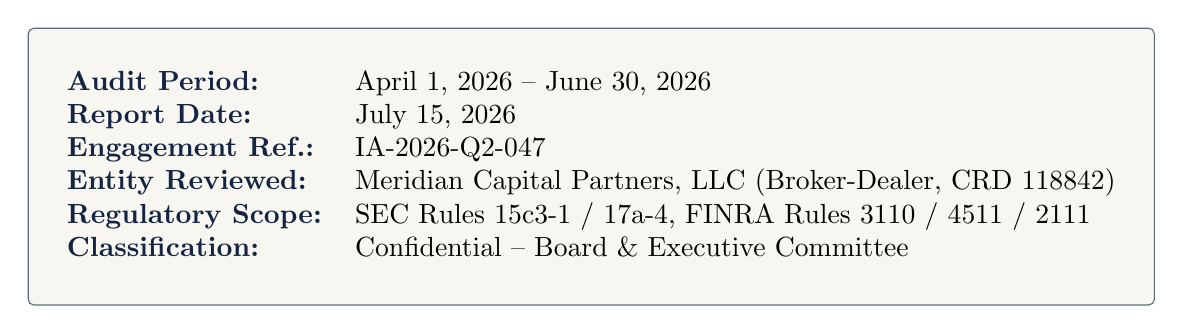
\begin{tikzpicture}
\node[draw=auditslate,fill=auditpaper,rounded corners=2pt,inner sep=14pt,align=left] (box) {%
\begin{tabular}{@{}ll@{}}
\textbf{\color{auditnavy}Audit Period:} & April 1, 2026 -- June 30, 2026 \\
\textbf{\color{auditnavy}Report Date:} & July 15, 2026 \\
\textbf{\color{auditnavy}Engagement Ref.:} & IA-2026-Q2-047 \\
\textbf{\color{auditnavy}Entity Reviewed:} & Meridian Capital Partners, LLC (Broker-Dealer, CRD 118842) \\
\textbf{\color{auditnavy}Regulatory Scope:} & SEC Rules 15c3-1 / 17a-4, FINRA Rules 3110 / 4511 / 2111 \\
\textbf{\color{auditnavy}Classification:} & Confidential -- Board \& Executive Committee \\
\end{tabular}%
};
\end{tikzpicture}
\end{center}

\vfill

\begin{center}
{\small\color{auditslate} Prepared by the Meridian Internal Audit \& Compliance Division\\
in coordination with Apex Risk Advisory (independent co-source reviewer)}
\end{center}

\vspace{0.6cm}
\begin{center}
\renewcommand{\arraystretch}{1.3}
\begin{tabular}{p{4.2cm}p{4.2cm}p{4.2cm}}
\centering\footnotesize\textbf{Rachel Donovan} & \centering\footnotesize\textbf{Marcus Whitfield} & \centering\footnotesize\textbf{Elena Petrova}\tabularnewline
\centering\scriptsize Chief Compliance Officer & \centering\scriptsize Director, Internal Audit & \centering\scriptsize Head of Risk Management\tabularnewline
\end{tabular}
\end{center}
\end{titlepage}

%----------------------------------------------------------------------
\chapter*{Confidential Audit Report}
\addcontentsline{toc}{chapter}{Confidential Audit Report}

\section*{Executive Summary}

The Meridian Internal Audit \& Compliance Division completed its Q2~2026 review of the firm's
risk management and regulatory compliance program, covering anti-money-laundering (AML)
controls, net capital computation, Regulation Best Interest (Reg~BI) supervision, books and
records retention, business continuity planning, and governance/supervisory controls. The
review was performed under the Institute of Internal Auditors (IIA) International Standards
and incorporated targeted testing co-sourced with Apex Risk Advisory.

\begin{center}
\begin{minipage}{0.47\linewidth}
\begin{ratingbox}{riskmed}{Overall Program Rating}
\centering
{\Huge\bfseries\color{riskmed} 80\,/\,100}\\[4pt]
{\small\color{auditslate} \textbf{Needs Improvement} -- controls are largely designed
adequately but two areas carry elevated exposure requiring remediation before the Q3
FINRA cycle exam.}
\end{ratingbox}
\end{minipage}\hfill
\begin{minipage}{0.47\linewidth}
\begin{ratingbox}{auditnavy}{Findings Snapshot}
\centering
\begin{tabular}{@{}ccc@{}}
\textcolor{riskhigh}{\Large\bfseries 2} & \textcolor{riskmed}{\Large\bfseries 2} & \textcolor{risklow}{\Large\bfseries 2}\\
{\scriptsize High} & {\scriptsize Medium} & {\scriptsize Low}
\end{tabular}\\[4pt]
{\small\color{auditslate} 6 findings total -- 0 carried forward from Q1~2026}
\end{ratingbox}
\end{minipage}
\end{center}

\vspace{0.3cm}
\noindent Composite scores by control area, based on design effectiveness and testing results
(sample sizes detailed in Section~2):

\begin{center}
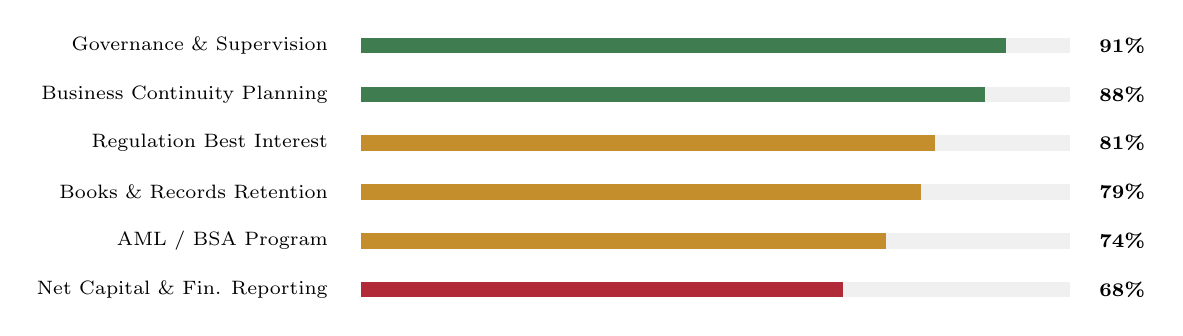
\begin{tikzpicture}[y=0.62cm,x=1cm]
\barrow{Governance \& Supervision}{91}{risklow}{6}
\barrow{Business Continuity Planning}{88}{risklow}{5}
\barrow{Regulation Best Interest}{81}{riskmed}{4}
\barrow{Books \& Records Retention}{79}{riskmed}{3}
\barrow{AML / BSA Program}{74}{riskmed}{2}
\barrow{Net Capital \& Fin. Reporting}{68}{riskhigh}{1}
\end{tikzpicture}
\end{center}

%----------------------------------------------------------------------
\section*{Scope \& Methodology}

The audit assessed the design and operating effectiveness of controls supporting Meridian's
obligations under SEC Rule 15c3-1 (net capital), SEC Rule 17a-4 (books and records), FINRA
Rule 3110 (supervision), FINRA Rule 4511 (recordkeeping), and FINRA Rule 2111 / Regulation
Best Interest. Fieldwork combined walkthroughs, control re-performance, and system-generated
evidence pulled directly from Meridian's internal platforms:

\begin{itemize}[leftmargin=1.4em,itemsep=2pt]
  \item[\faFile] \textbf{Vertex} -- order management and trade surveillance system of record
  \item[\faUsers] \textbf{Synapse} -- client onboarding, KYC, and CIP evidence repository
  \item[\faLock] \textbf{Nexa Prime} -- core brokerage ledger and net capital calculation engine
  \item[\faChartLine] \textbf{Nimbus Cloud} -- infrastructure and disaster-recovery hosting provider
\end{itemize}

Sampling followed a risk-based approach: high-risk populations (AML alerts, margin
exceptions) were tested at 100\% for the quarter; medium-risk populations used statistically
valid samples ($n \geq 25$, 95\% confidence, 5\% tolerable exception rate); low-risk
populations were tested judgmentally.

%----------------------------------------------------------------------
\section*{Risk Heat Map}

Findings are plotted below by likelihood of recurrence and potential regulatory / financial
impact, consistent with Meridian's Enterprise Risk Management framework.

\begin{center}
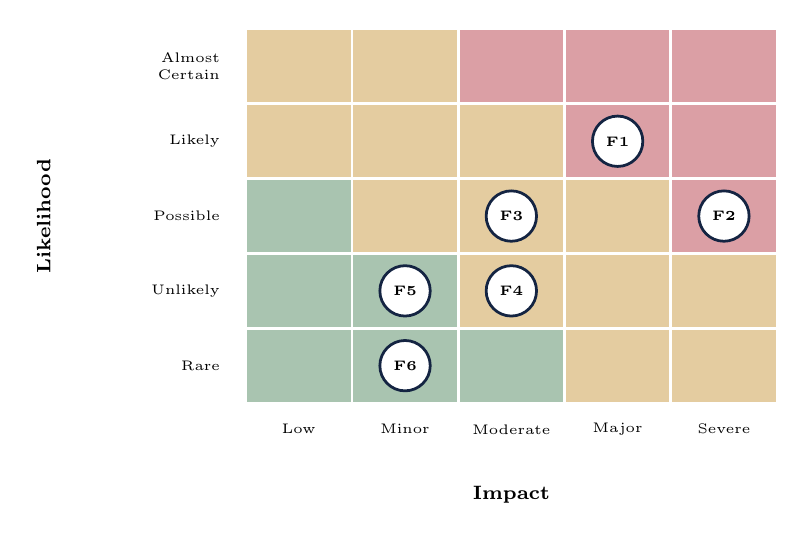
\begin{tikzpicture}[x=1.35cm,y=0.95cm,every node/.style={font=\tiny}]
  % background grid
  \foreach \x in {0,...,4}{
    \foreach \y in {0,...,4}{
      \pgfmathtruncatemacro{\s}{\x+\y}
      \ifnum\s<3
        \draw[fill=risklow!45,draw=white,line width=1pt] (\x,\y) rectangle ++(1,1);
      \else
        \ifnum\s<6
          \draw[fill=riskmed!45,draw=white,line width=1pt] (\x,\y) rectangle ++(1,1);
        \else
          \draw[fill=riskhigh!45,draw=white,line width=1pt] (\x,\y) rectangle ++(1,1);
        \fi
      \fi
    }
  }
  % axes labels
  \foreach \x/\lab in {0/Low,1/Minor,2/Moderate,3/Major,4/Severe}{
    \node at (\x+0.5,-0.35) {\lab};
  }
  \foreach \y/\lab in {0/Rare,1/Unlikely,2/Possible,3/Likely,4/Almost Certain}{
    \node[anchor=east,text width=1.5cm,align=right] at (-0.15,\y+0.5) {\lab};
  }
  \node[font=\scriptsize\bfseries,below=0.6cm] at (2.5,-0.35) {Impact};
  \node[font=\scriptsize\bfseries,rotate=90] at (-1.9,2.5) {Likelihood};

  % finding markers
  \node[circle,draw=auditnavy,fill=white,minimum size=16pt,line width=1pt] at (3.5,3.5) {\tiny\bfseries F1};
  \node[circle,draw=auditnavy,fill=white,minimum size=16pt,line width=1pt] at (4.5,2.5) {\tiny\bfseries F2};
  \node[circle,draw=auditnavy,fill=white,minimum size=16pt,line width=1pt] at (2.5,2.5) {\tiny\bfseries F3};
  \node[circle,draw=auditnavy,fill=white,minimum size=16pt,line width=1pt] at (2.5,1.5) {\tiny\bfseries F4};
  \node[circle,draw=auditnavy,fill=white,minimum size=16pt,line width=1pt] at (1.5,1.5) {\tiny\bfseries F5};
  \node[circle,draw=auditnavy,fill=white,minimum size=16pt,line width=1pt] at (1.5,0.5) {\tiny\bfseries F6};
\end{tikzpicture}
\end{center}

%----------------------------------------------------------------------
\section*{Compliance Testing Results}

\rowcolors{2}{white}{auditpaper!70}
\begin{center}
\begin{tabularx}{\linewidth}{@{}p{3.4cm}Xccc@{}}
\toprule
\rowcolor{auditnavy}
\textcolor{white}{\textbf{Regulatory Area}} & \textcolor{white}{\textbf{Test Performed}} &
\textcolor{white}{\textbf{Sample}} & \textcolor{white}{\textbf{Exceptions}} & \textcolor{white}{\textbf{Result}} \\
\midrule
AML / BSA (FINRA 3310) & CDD escalation timeliness on flagged Synapse alerts & 100\% (Q2) & 6 & \textcolor{riskmed}{\bfseries Partial} \\
Net Capital (SEC 15c3-1) & Reconciliation of Nexa Prime ledger to net capital filing & 12 filings & 3 & \textcolor{riskhigh}{\bfseries Fail} \\
Reg BI (FINRA 2111) & Disclosure Form CRS delivery \& documentation & 30 accounts & 4 & \textcolor{riskmed}{\bfseries Partial} \\
Books \& Records (17a-4) & WORM configuration on Synapse retained records & 40 records & 5 & \textcolor{riskmed}{\bfseries Partial} \\
Business Continuity & BCP annual test execution \& sign-off & 1 cycle & 1 & \textcolor{risklow}{\bfseries Pass*} \\
Supervision (FINRA 3110) & OBA disclosure logging in Vertex compliance module & 22 reps & 2 & \textcolor{risklow}{\bfseries Pass*} \\
\bottomrule
\end{tabularx}
\end{center}
{\footnotesize\color{auditslate}*Pass with minor exceptions noted -- see Findings F5 and F6.}

%----------------------------------------------------------------------
\section*{Detailed Findings}

\begin{tcolorbox}[colback=riskhigh!6,colframe=riskhigh,arc=2pt,boxrule=0.9pt,left=8pt,right=8pt,top=5pt,bottom=5pt,breakable]
\textbf{F1 -- AML Exception Handling Delays} \hfill \severitytag{3}\\[3pt]
\textit{Condition:} Six of six sampled Synapse AML alerts requiring enhanced due diligence
were escalated to the BSA Officer more than 5 business days after generation (policy
requires 2 days); average delay was 7.4 days.\\
\textit{Cause:} The alert queue lacks an automated SLA countdown, and the sole reviewer
covering EDD escalations was on leave for three weeks during the quarter with no backup
assigned.\\
\textit{Impact:} Delayed escalation increases the risk of undetected suspicious activity and
exposes the firm to FINRA Rule 3310 deficiency findings.\\
\textit{Recommendation:} Configure automated SLA alerts in Synapse and cross-train a second
BSA analyst as backup reviewer.
\end{tcolorbox}

\vspace{4pt}
\begin{tcolorbox}[colback=riskhigh!6,colframe=riskhigh,arc=2pt,boxrule=0.9pt,left=8pt,right=8pt,top=5pt,bottom=5pt,breakable]
\textbf{F2 -- Net Capital Reconciliation Gap} \hfill \severitytag{3}\\[3pt]
\textit{Condition:} Three of twelve monthly net capital filings showed unreconciled
variances between the Nexa Prime ledger and the filed FOCUS report, ranging from \$41,000 to
\$118,000, with no documented explanation retained.\\
\textit{Cause:} A manual journal-entry adjustment step in the month-end close is not
captured by the automated reconciliation script introduced in Q4~2025.\\
\textit{Impact:} Unreconciled variances create risk of an inaccurate net capital
computation and potential SEC Rule 15c3-1 early-warning notification failure.\\
\textit{Recommendation:} Extend the reconciliation script to ingest manual journal entries
and require CFO sign-off on any variance exceeding \$10,000 before filing.
\end{tcolorbox}

\vspace{4pt}
\begin{minipage}{0.485\linewidth}
\begin{tcolorbox}[colback=riskmed!6,colframe=riskmed,arc=2pt,boxrule=0.9pt,left=7pt,right=7pt,top=5pt,bottom=5pt]
\textbf{\small F3 -- Reg BI Disclosure Gaps} \hfill \severitytag{2}\\[2pt]
{\footnotesize 4 of 30 sampled accounts lacked a dated, signed Form~CRS acknowledgment in
Synapse at account opening. Recommend a hard system gate blocking trade entry until Form
CRS delivery is confirmed.}
\end{tcolorbox}
\end{minipage}\hfill
\begin{minipage}{0.485\linewidth}
\begin{tcolorbox}[colback=riskmed!6,colframe=riskmed,arc=2pt,boxrule=0.9pt,left=7pt,right=7pt,top=5pt,bottom=5pt]
\textbf{\small F4 -- Records Retention (WORM)} \hfill \severitytag{2}\\[2pt]
{\footnotesize 5 of 40 sampled Synapse records were stored on rewritable volumes rather than
the WORM-compliant archive required by SEC Rule 17a-4(f). Recommend migrating the affected
document classes and auditing storage policy quarterly.}
\end{tcolorbox}
\end{minipage}
\par
\vspace{6pt}
\begin{minipage}{0.485\linewidth}
\begin{tcolorbox}[colback=risklow!6,colframe=risklow,arc=2pt,boxrule=0.9pt,left=7pt,right=7pt,top=5pt,bottom=5pt]
\textbf{\small F5 -- BCP Test Documentation} \hfill \severitytag{1}\\[2pt]
{\footnotesize The FY2026 business continuity test executed on schedule via Nimbus Cloud
failover, but the after-action report was not signed off by the Business Continuity
Committee within the required 10-day window.}
\end{tcolorbox}
\end{minipage}\hfill
\begin{minipage}{0.485\linewidth}
\begin{tcolorbox}[colback=risklow!6,colframe=risklow,arc=2pt,boxrule=0.9pt,left=7pt,right=7pt,top=5pt,bottom=5pt]
\textbf{\small F6 -- OBA Disclosure Logging} \hfill \severitytag{1}\\[2pt]
{\footnotesize 2 of 22 sampled representatives had outside business activities approved via
email but not logged in the Vertex compliance module, creating an incomplete supervisory
record.}
\end{tcolorbox}
\end{minipage}
\par

%----------------------------------------------------------------------
\section*{Remediation Plan}

\rowcolors{2}{white}{auditpaper!70}
\begin{center}
\begin{tabularx}{\linewidth}{@{}cXlll@{}}
\toprule
\rowcolor{auditnavy}
\textcolor{white}{\textbf{ID}} & \textcolor{white}{\textbf{Finding}} & \textcolor{white}{\textbf{Owner}} &
\textcolor{white}{\textbf{Target Date}} & \textcolor{white}{\textbf{Status}} \\
\midrule
F1 & AML exception handling delays & R. Donovan (CCO) & Aug 15, 2026 & \textcolor{riskhigh}{In Progress} \\
F2 & Net capital reconciliation gap & CFO Office & Aug 31, 2026 & \textcolor{riskhigh}{In Progress} \\
F3 & Reg BI disclosure gaps & E. Petrova (Risk) & Sep 15, 2026 & \textcolor{riskmed}{Open} \\
F4 & WORM records retention & IT / Synapse Admin & Sep 30, 2026 & \textcolor{riskmed}{Open} \\
F5 & BCP sign-off documentation & M. Whitfield (IA) & Aug 1, 2026 & \textcolor{risklow}{Open} \\
F6 & OBA disclosure logging & Supervision Team & Aug 15, 2026 & \textcolor{risklow}{Open} \\
\bottomrule
\end{tabularx}
\end{center}

\noindent{\footnotesize\color{auditslate} Findings F1 and F2 are designated \textbf{high
priority} and will be re-tested by Internal Audit prior to the Q3~2026 FINRA cycle exam
window. All remediation owners are required to submit interim status updates to the Audit
Committee at each monthly compliance meeting.}

%----------------------------------------------------------------------
\section*{Sign-Off}

\begin{center}
\renewcommand{\arraystretch}{1.3}
\begin{tabular}{p{5cm}p{5cm}p{4cm}}
\hrulefill & \hrulefill & \hrulefill \\
\footnotesize Rachel Donovan, Chief Compliance Officer & \footnotesize Marcus Whitfield, Director of Internal Audit & \footnotesize Date \\
\end{tabular}
\end{center}

\vspace{0.15cm}
\begin{center}
{\footnotesize\color{auditslate} This report and its contents are confidential and intended
solely for the Meridian Capital Partners Audit Committee and Executive Management. Distribution
outside these parties requires prior written authorization from the Chief Compliance Officer.}
\end{center}

\end{document}
